\documentclass{article}

\usepackage[left=2.5cm, right=2.5cm, top=2.5cm, bottom=2.5cm]{geometry}
\usepackage{graphicx}
\usepackage{physics}
\usepackage{subcaption}
\usepackage{hyperref}
\usepackage{caption}
\captionsetup{width=.9\textwidth}
\usepackage[version=4]{mhchem}



\title{Exercise 3, TFY4235 Computational physics}
\author{Martin Johnsrud}
\vspace{-8ex}
\date{}


\begin{document}
    \maketitle
    \section*{Introduction}
        This is an implementation of \cite{exercise}.
    \section*{Theory and implementation}
    The diffusion equation, can be written as
    \begin{equation*}
        \Delta t \pdv{t} C(z, t) = \Delta t \left(K(z) \pdv[2]{z} + \dv{K(z)}{z}\pdv{z}\right) C(z, t) = \mathcal{D} C(z, t).
    \end{equation*}
    Discretizing the spatial part, and applying boundary conditions, gives
    \begin{equation*}
        \Delta t \pdv{t} C_n(t) = \mathcal{D}_{nm} C_n(t) + S_n(t),
    \end{equation*}
    where 
    \begin{align*}
        \mathcal{D} &=
        \begin{pmatrix}
            -4\alpha K_0 - 2\Gamma & 4\alpha K_0 & 0 & \dots&0 \\
            -\frac{\alpha}{2} K_1' + 2\alpha K_1 & -4 \alpha K_1 & \frac{\alpha}{2}K_1' + 2\alpha K_1 &  \dots & 0 \\
            0 & \ddots & \ddots & \ddots & 0\\
            0 & \dots &-\frac{\alpha}{2} K_{N-1}' + 2\alpha K_{N-1} & -4 \alpha K_{N-1} & \frac{\alpha}{2}K_{N-1}' + 2\alpha K_{N-1} \\
             0 & \dots & 0 & 4\alpha K_N & -4\alpha K_N
        \end{pmatrix},\\
        S(t) & =  
        \begin{pmatrix}
            2\Gamma C_\mathrm{eq}(t) &0&\dots&0
        \end{pmatrix}^T \quad 
    \Gamma = 2 \frac{\alpha k_w \Delta z}{K_0} \left(K_0 - \frac{1}{2}(-\frac{3}{2} K_0 + 2K_1 - \frac{1}{2}K_2)\right), \quad
     \alpha = \frac{\Delta t}{2 \Delta z^2 },\\
      K_n' & = K_{n+1} - K_{n-1}
    \end{align*}
    The Cranck-Nichelson scheme then yields
    \begin{equation*}
        C_n^{i+1}  = C_n^i + \frac{1}{2} (\mathcal{D}_{nm} C_m^i + S_n^i) + \frac{1}{2} (\mathcal{D}_{nm} C_m^{i+1} + S_n^{i+1}),
    \end{equation*}
    so the equation to be solved to get the next timestep is
    \begin{align*}
        & A_{nm} C_{m}^{i+1} = V_n^i, \\ 
        & V_n^i = \left(\delta_{nm} + \frac{1}{2} \mathcal{D}_{nm}\right) C_m^i + \frac{1}{2}(S_n^i + S_n^{i+1}), \quad 
        A_{mn} = \left(\delta_{nm} - \frac{1}{2} \mathcal{D}_{nm}\right)
    \end{align*}
    
    The implementation of this system of equation uses SciPy's sparse matrix library. After creating sparse realizations of $A$, SciPy's \verb|splu| is used to generate the LU decomposition \verb|LU| of $A$. This is an object with methods such as \verb|.solve()|, which utilizes the LU decomposition. The wrapper \verb|simulate| then loops over $N_t-1$ steps, using \verb|solve(V) = lambda V: LU.solve(V)|, where \verb|V| is as given above. 

    \section*{Tests}
    Make sure the implementation gives good answers, it is compared to known solutions. The method used in this implementation has quadratic convergence, both in time and space. A convergence test was implemented for a simple test case, to check this. \autoref{convergence test} shows the result of this. 

    \begin{figure}
        \centering
        \includegraphics[width=.49\textwidth]{../plots/conv_test}
        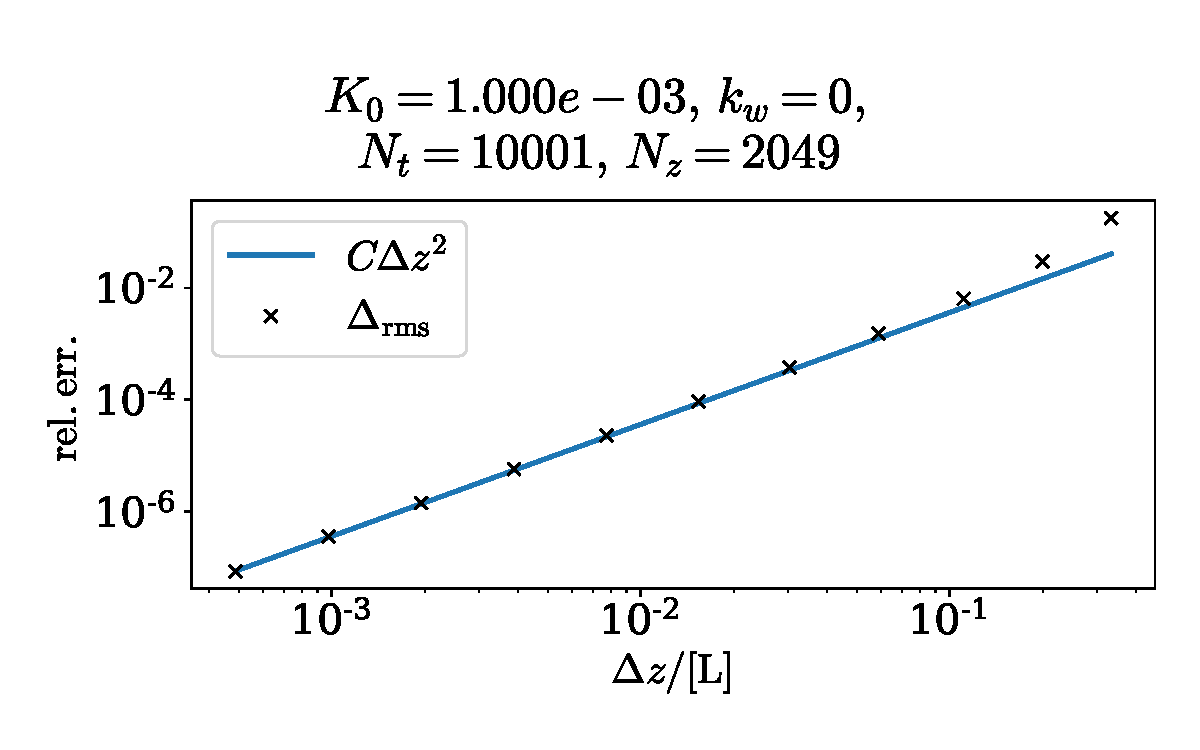
\includegraphics[width=.49\textwidth]{../plots/conv_test_z}
        \caption{Error, measured as the root mean square deviation from a reference value, after 1 day simulation of an gaussian initial concentration.}
        \label{convergence test}
    \end{figure}

    A constant concentration of \ce{CO2} should remain constant, regardless of $K(z)$, as long as it is positive. This test is shown in \autoref{constant_cons}, with a both a constant $K(z)$, and a smooth step function between two values of $K$. For both, the constant initial concentration is close to unchanged, save for numerical errors.

    \begin{figure}
        \centering
        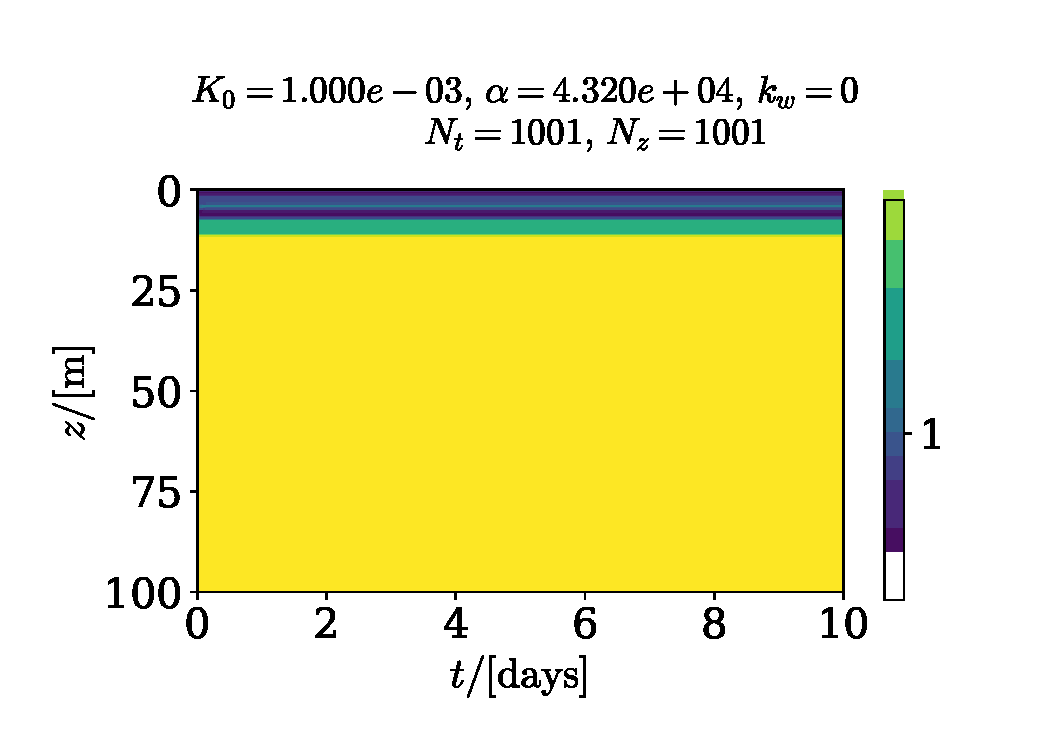
\includegraphics[width=.49\textwidth]{../plots/test1}
        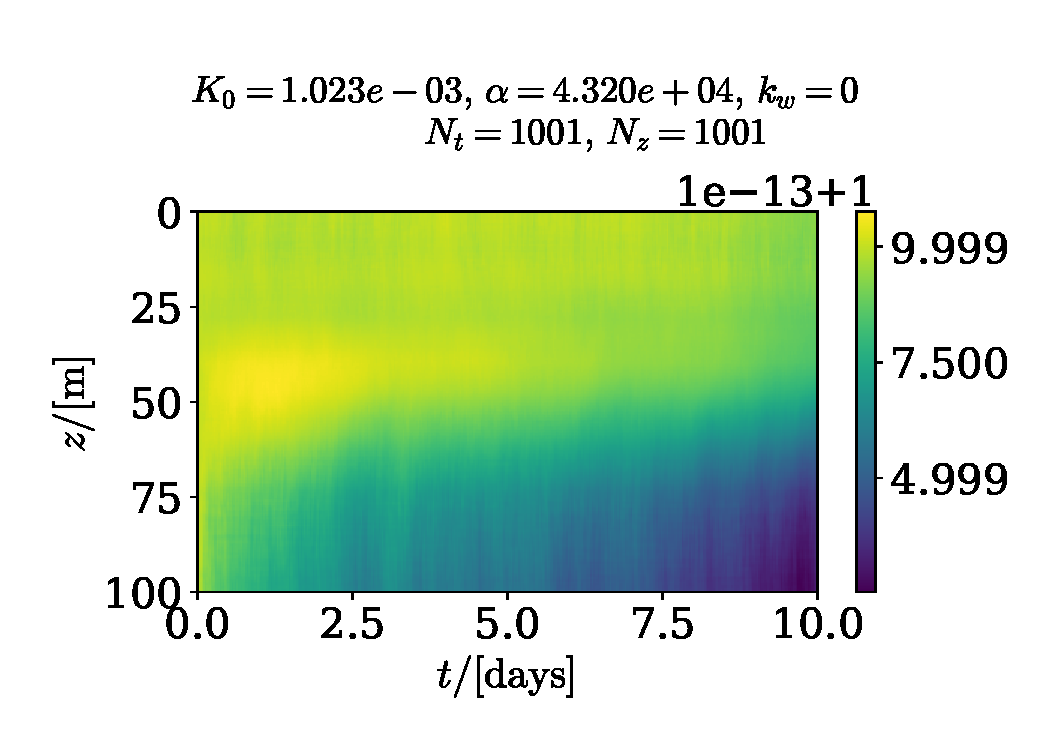
\includegraphics[width=.49\textwidth]{../plots/test1_varK}
        \caption{The time evolution of an constant concentration. The system on the left has a constant $K(z)$, while system of the right has an oscillatory $K$. The largest deviation of the system is of order $10^{-16}$ and $10^{-15}$, respectively.}
        \label{constant_cons}
    \end{figure}

    The systems should also, given $k_w=0$, conserve mass. To test this, a initial distribution of two gaussian functions were evolved in time, with a non-constant diffusivity. The result is shown in \autoref{Consv mass}, where the mass is conserved to a good approximation.

    \begin{figure}
        \centering
        \includegraphics[width=.49\textwidth]{../plots/test2_c}
        \includegraphics[width=.49\textwidth]{../plots/test2_m}
        \caption{The evolution of a gaussian distribution of \ce{CO2} is shown on the left. On the right, the relative change in mass as a function of time is plotted. }
        \label{Consv mass}
    \end{figure}

    A sharply peaked gaussian package should have a variance that increases linearly with time, then approach a steady state. This is shown in \autoref{var}.

    \begin{figure}
        \centering
        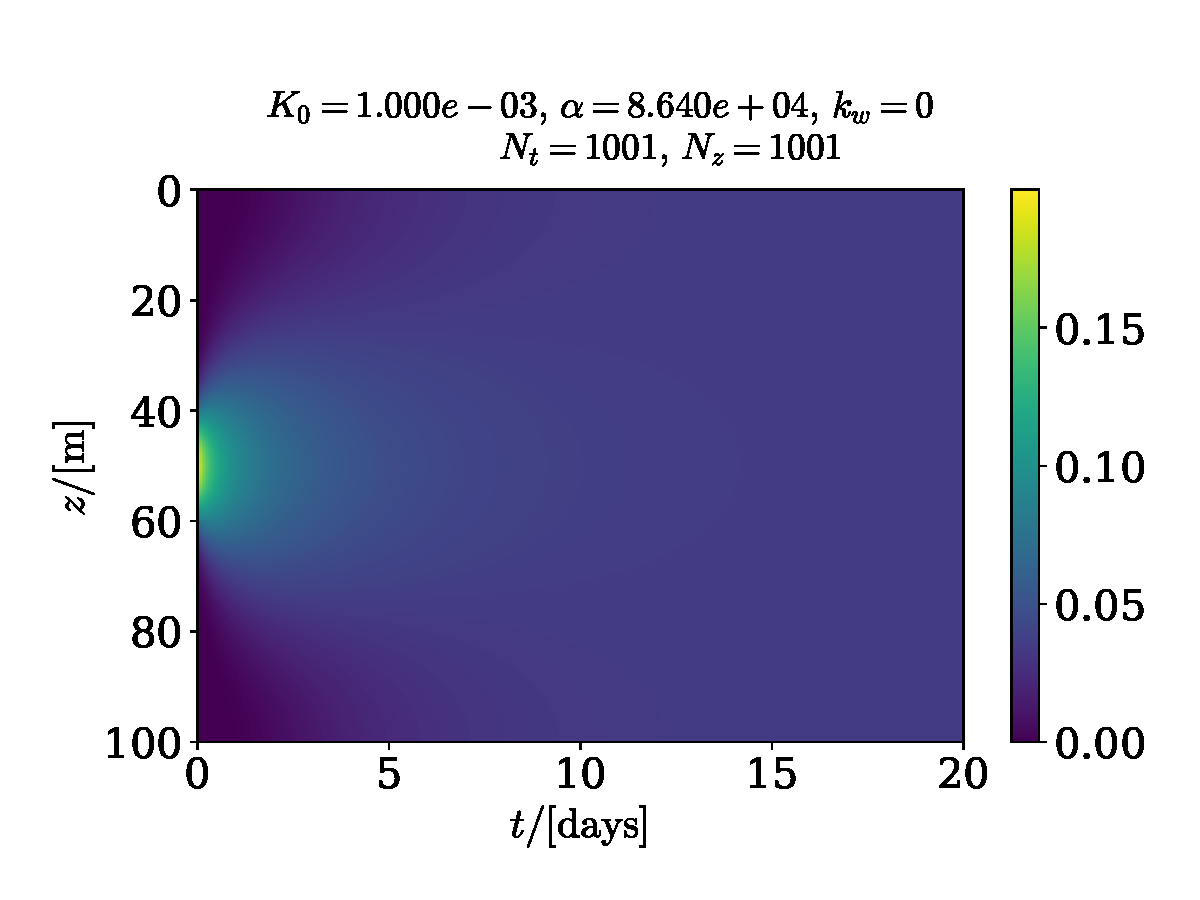
\includegraphics[width=.49\textwidth]{../plots/test3}
        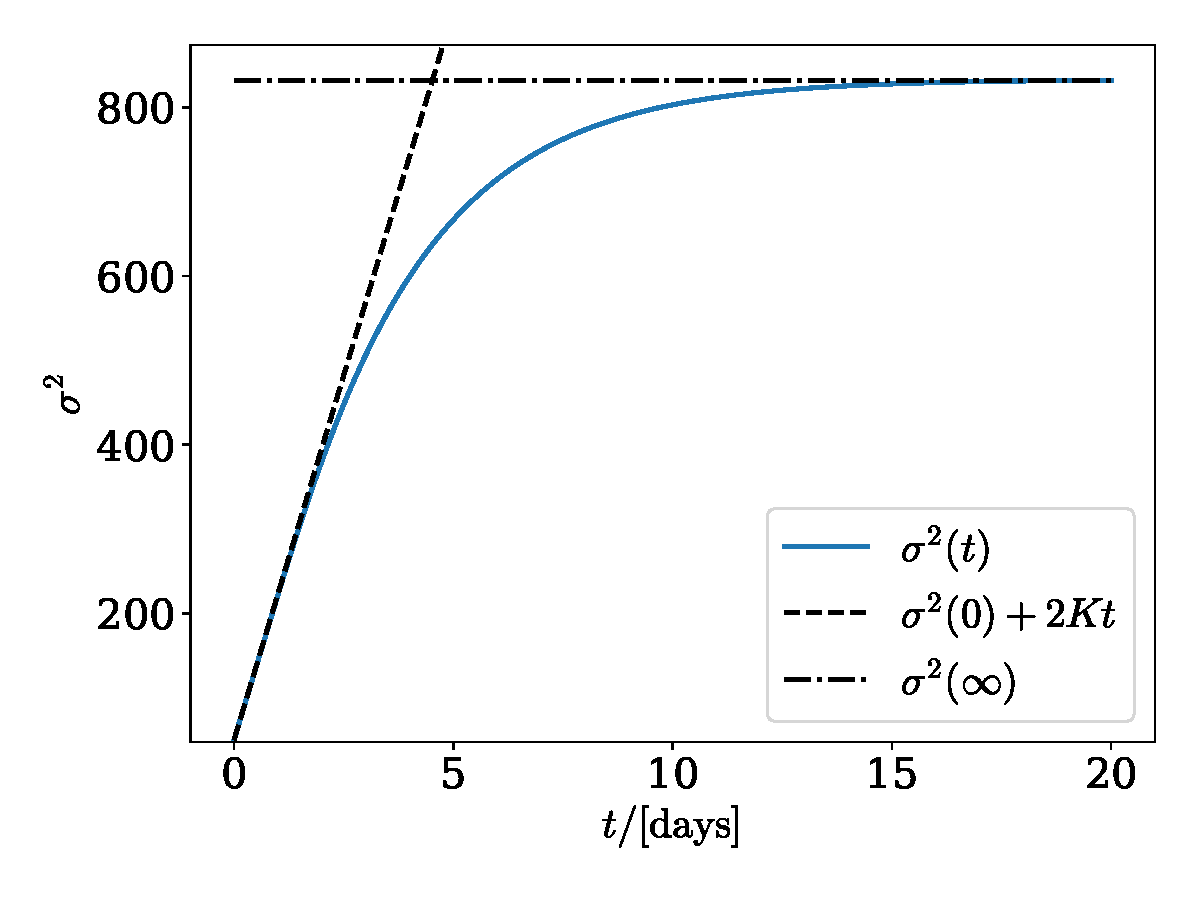
\includegraphics[width=.49\textwidth]{../plots/test3_var}
        \caption{}
        \label{var}
    \end{figure}

    \autoref{decay} shows the depletion of \ce{CO2} from the ocean, given a zero partial pressure in the atmosphere. For a small Biot number, this should follow a exponential decay, as this test shows.

    \begin{figure}
        \centering
        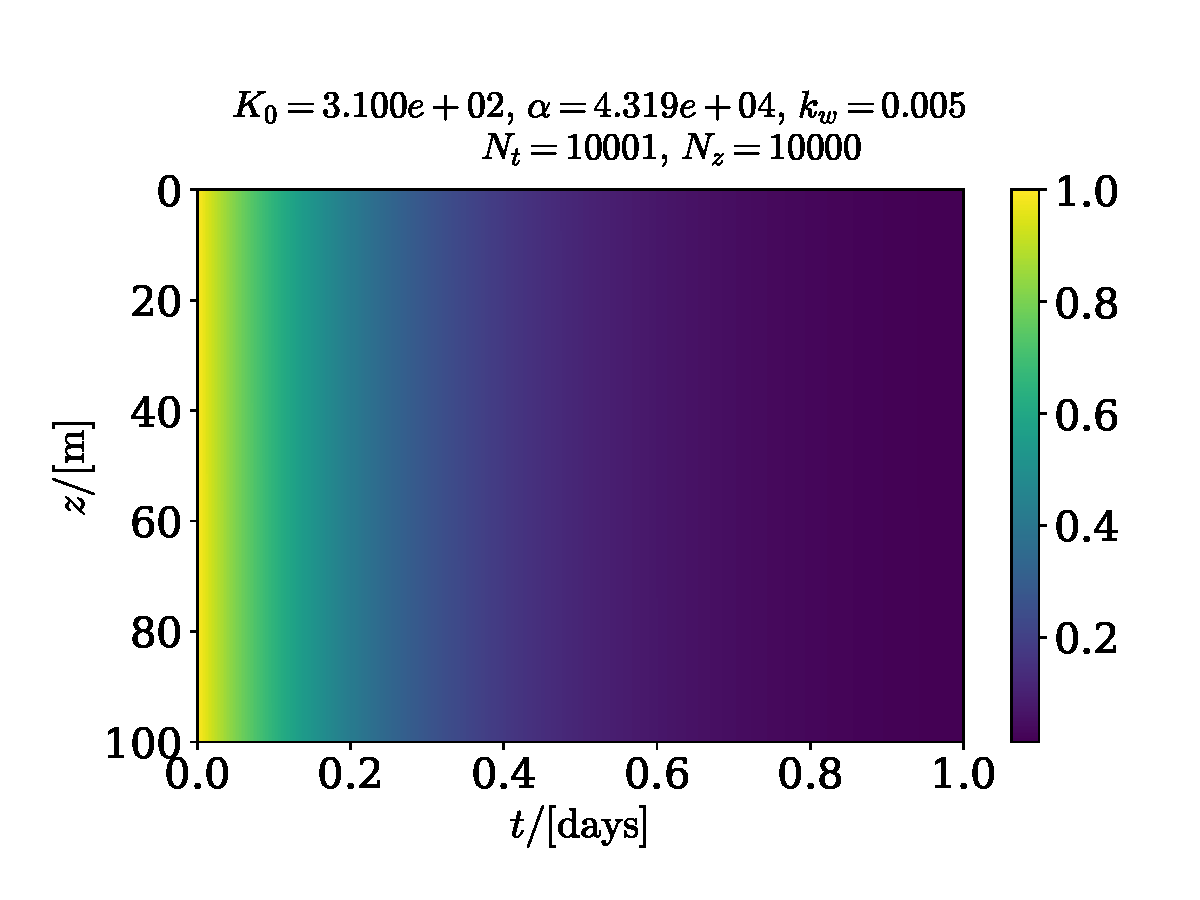
\includegraphics[width=.49\textwidth]{../plots/test4}
        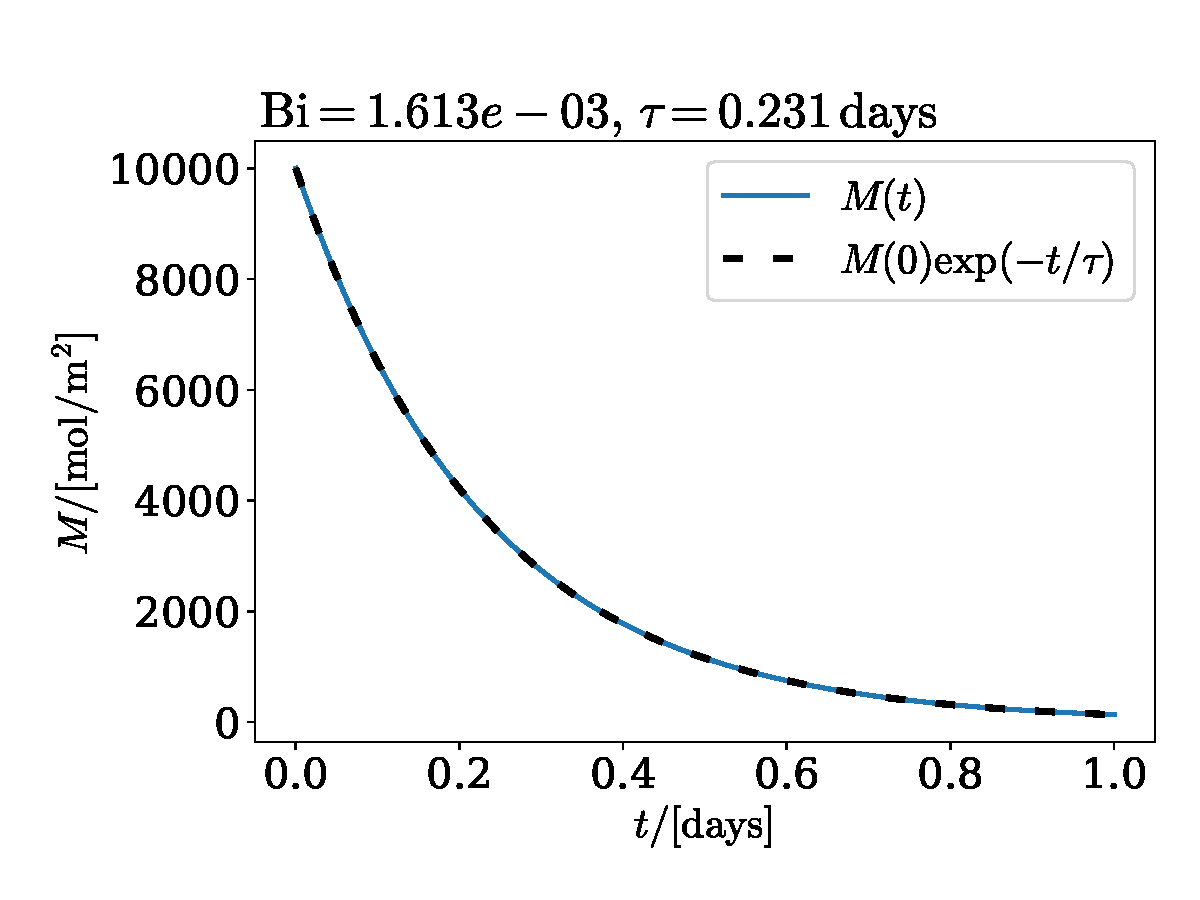
\includegraphics[width=.49\textwidth]{../plots/test4_decay}
        \caption{The slow removal of \ce{CO2} from the ocean, when the atmosphere contains a partial pressure of 0.}
        \label{decay}
    \end{figure}

    Lastly, \autoref{minmax} shows how the ocean reaches a equilibrium with the atmosphere, given a non-zero, positive mass-transfer coefficient $k_w$ and either constant or non-constant diffusivity.

    \begin{figure}
        \centering
        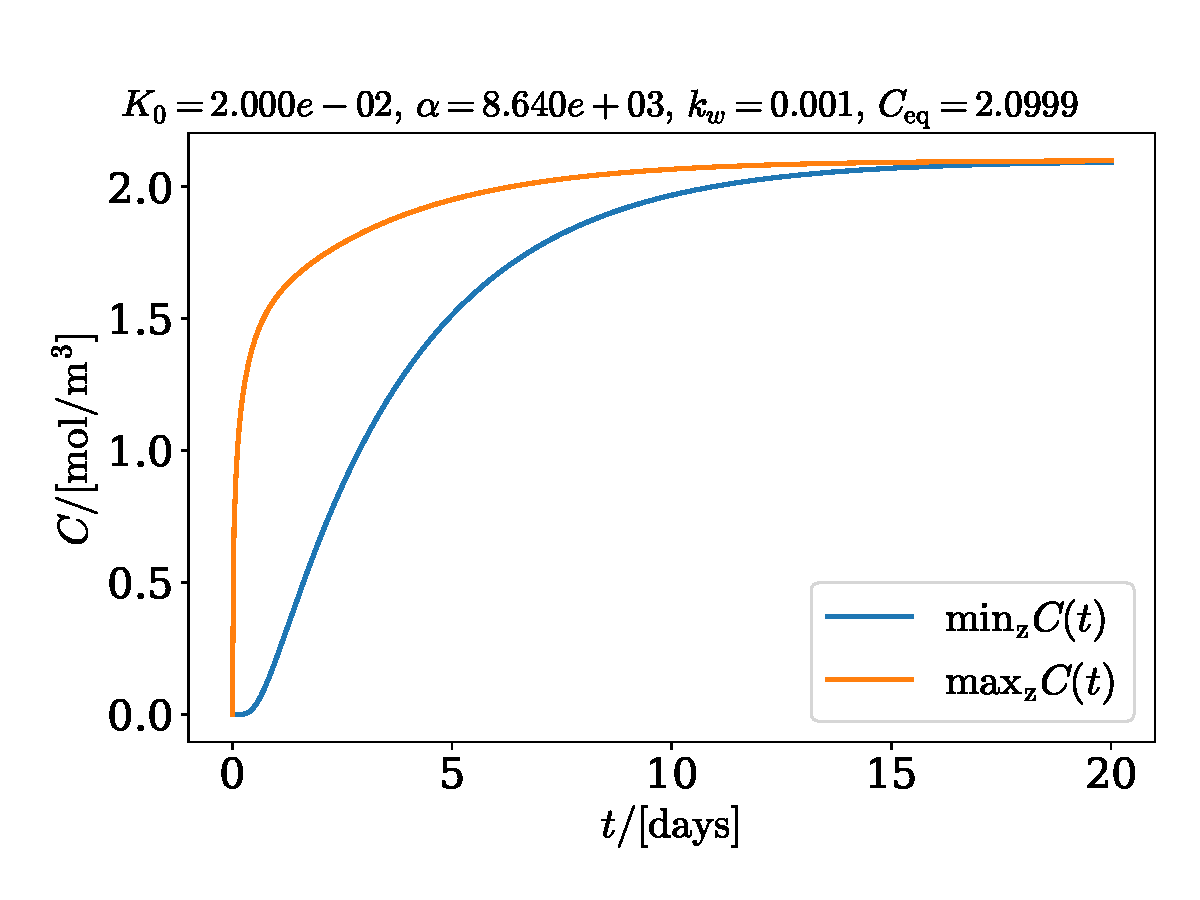
\includegraphics[width=.49\textwidth]{../plots/test5_minmax}
        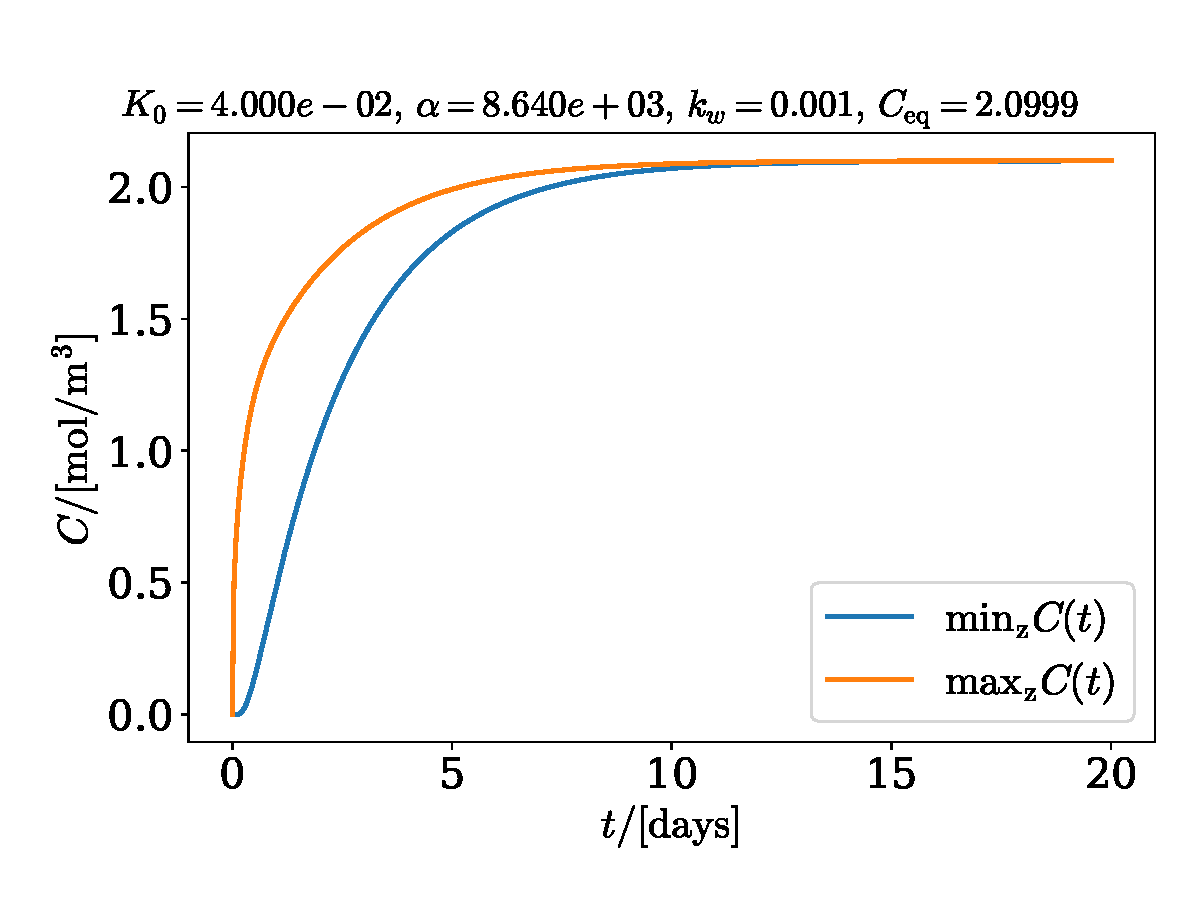
\includegraphics[width=.49\textwidth]{../plots/test5_varK_minmax}
        \caption{Equilibration of the ocean with a atmosphere with $C_\mathrm{eq}=0.5$. The figure on the left is a system with constant diffusivity, the left side has a oscillating but always positive diffusivity.}
        \label{minmax}
    \end{figure}

    \bibliography{report}
    \bibliographystyle{plain}

\end{document}